\chapter{時系列UX評価システムの提案}
\label{chap:sequential}

本章では,時系列UX評価システムの設計及び実装と,その妥当性を検討するために行った実験について述べる.第\ref{chap:pulsewave}章で述べた満足性とANB,LLE,HRの関連性を調査した実験では,満足性とANBとの関連性が明らかになった.そこで,ANBの変化を時系列の満足性変化として捉え,UXを評価するシステムを開発した.また,LLEとHRについては前述の実験では満足性との関係性を明らかにできなかったものの,短いスパンでの代表値として利用することで有効に活用できる可能性がある.そのため,短時間のBVPから計算したLLEと瞬間のHRであるRRIについても計測した.

\section{設計}

時系列UX評価システムのプロトタイプとして主要な部分のみを実装した.本研究において時系列UX評価とは,システムの使用時,使用前,使用後,使用していない期間のUXを,何らかの指標やユーザの自己申告などに基づいてその変化を可視化することを指す.従来手法としてはUXグラフなどがあるが,ここでは特に使用時のUX変化をより短いタイムスパンで表示することを対象とする.

使用時の時系列UX評価において重要なのは,指標を用いて詳細なグラフを表示することと,そのグラフを実際のユーザの動作と対応づけることである.この2点を実現するためのシステムを開発した.

\subsection{使用時UXグラフの表示}

使用時UXグラフを表示するための指標としてANB,LLE,RRIを採用しこれらを同時に表示するシステムを開発した.従来のUXグラフではユーザの自己申告によって手描きで満足度の変化をグラフに書き起こしていた.しかし,使用時の秒単位での変化を使用時に書いてもらったり,使用後に書いてもらうことは難しい.そこで生体データから得られるストレスに関する指標を満足性を表す値として使用する.具体的には前述のように満足性との関連が見られたANBと,有意差は見られなかったものの短いスパンにすることで活用できる可能性があるLLE,RRIを指標として採用した.

ストレスを測定するためにPPGを使用しBVPを記録する.測定には,耳朶用の光学式容積脈波計であるVital Meter with 3D Accelerometer(製造:TAOS Institute, Inc.,図\ref{fig:device1})を使用し1000Hzでサンプリングした.なお,測定器側で適切なフィルタリングがかけられていることを確認し,記録した波形はフィルタリング済みのものである.また,分析にANB,LLE,RRIの分析にあたっては200Hzにダウンサンプリングしたデータを使用した.第\ref{chap:pulsewave}章で行った研究では指先用のセンサを使用したがここでは耳朶に装着するものを使用した.これにより,手による操作が阻害されることがなくなりより正確なデータが得られるようになった.また,Vital MeterはBluetoothでコンピュータと接続するため被験者の姿勢や場所に制約が少なくなった.

ANBは0.15-4HzのHFと0.004Hz-0.15HzのLF成分から算出される値である.このことから,LF成分の周期は6.6-250秒であり,これを分析するためには最低でもそれを十分に捉えられるだけの長さの波から計算する必要があり,100拍,約5分間以上の測定が標準とされている\cite{yamaguchi}.そこで,時系列のANB分析では,256秒(4.26分)の波形からANBを算出し,10秒ずつスライドしながら算出を繰り返すことで,時系列のANBを取得した.なお,256秒に満たないデータからは簡易的に64秒の波からANBを算出することとした.

LLEはANBよりも短い時間の波から有効な値が得られることがわかっており,15秒の波形からLLEを算出し,ANBと同じく10秒ずつスライドしながら算出を繰り返すことで時系列のLLEを取得した.

RRIはANBの算出で使用する波のピーク位置を元にPeek to Peekの時間から瞬間心拍数を算出し1秒毎のRRIとした.

\subsection{使用時UXグラフとイベントのマッピング}

UXグラフでは,グラフの変化が大きい部分でどのようなイベントが起きていたのかを知ることが重要である.長期間のUXグラフでは,「使用の開始」「他の製品を使ったとき」などのイベントを先に提示し,イベントに対して満足性を記録することでグラフ化していた.しかし,使用時UXではグラフを見て問題がある部分のイベントを調査するという流れになると考えられる.

UXグラフと関連付けるイベントの取得には,使用の様子を動画で収録する,スクリーンキャプチャを取る,アプリケーションにログの記録機能を搭載するといった方法が考えられる.今回はプロトタイプであるため,またアプリケーションの種類を限定しないために使用の様子を動画で収録することとスクリーンキャプチャを取ることを採用した.

本研究では,休憩と実験毎をイベントとして分離すればよく,BVPの計測開始時刻を2つの動画と合致させたうえでBVPをそれぞれのイベント毎に分離するシステムを開発した.

\section{実装}

システムのフロントエンドはWebアプリケーションとして開発し,ANB,LLE,RRIを計算するエンジン部分はサーバーサイドアプリケーションとして開発した.

\subsection{脈波解析エンジン}

脈波の解析エンジンは,第\ref{chap:pulsewave}章の実験で使用したLyspectの開発元であるセレブラルダイナミックスから提供を受け,同一のものをサーバーサイドで実行できるようにした.システムはLyspectに準じてJavaで開発されており,Function as a Service\footnote{HTTPリクエストなどのイベントに応じて関数が実行されるサーバレスアーキテクチャ}であるGoogle Cloud Platform\footnote{Googleが提供するクラウドサービスの総称}のCloud Functionsでホスティングした.これにより,数秒から数十秒かかる解析であってもスケールアウト\footnote{コンピュータの台数を増やし処理を並列化・分散化させる手法.FaaSでは実際にコンピュータの台数が増えるとは限らないがインスタンスという形で仮想敵に台数が増えているといえる.}することで同時に多数の解析を実行することが可能になる.

エンジンにはREST APIを通じてアクセスできるため,ANB,LLE,RRIそれぞれのエンドポイントに200HzでサンプリングしたBVPをJSON形式で送ると数秒から数十秒後に解析の結果が返される.

\subsection{フロントエンド}

システムのフロントエンドはVue.jsを用いてWebアプリケーションとして開発した.このシステムでは,BVPの計測,RRI,LLE,ANBによる使用時UXグラフの表示,イベントとのマッピングを行うことができる.なお,プロトタイプであるためブラウザAPIのサポート状況の問題でWindowsまたはmacOSのChromeでしか動作を確認していない.

\begin{figure}[htbp]
  \begin{minipage}{\hsize}
    \begin{center}
       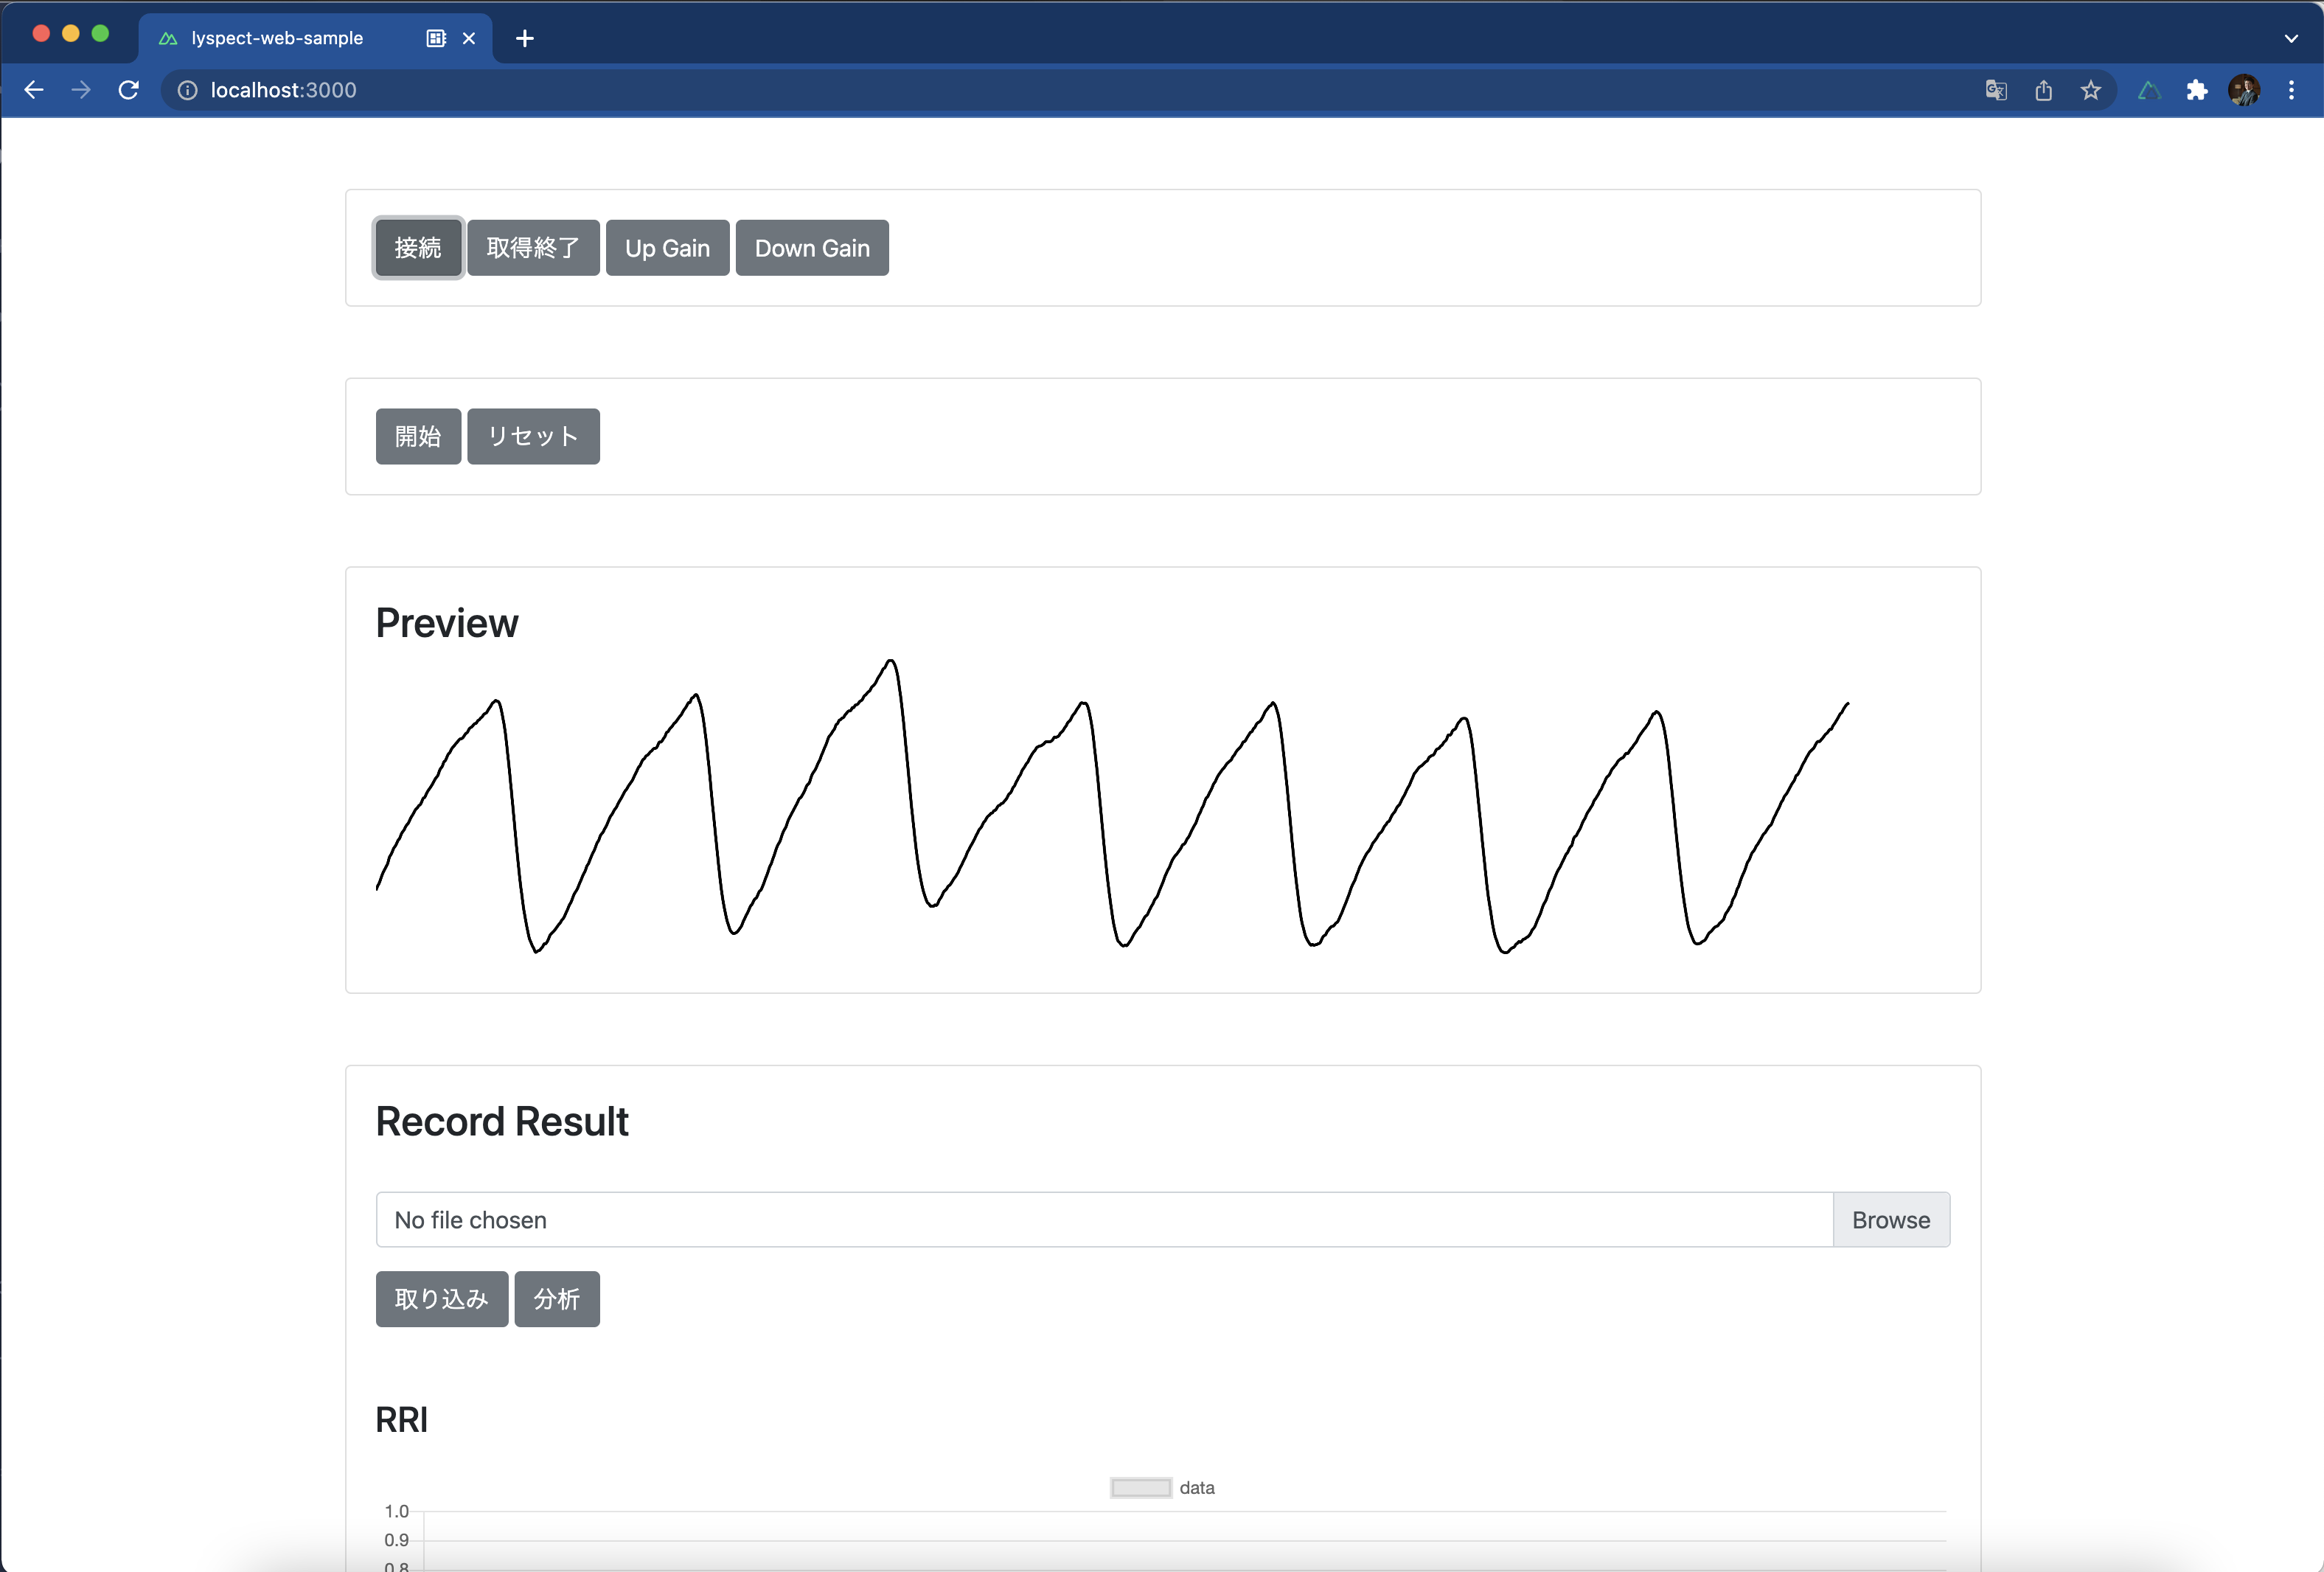
\includegraphics[width=100mm]{img/pwm.png}
    \end{center}
    \caption{脈波の計測画面}
    \label{fig:majorment}
  \end{minipage}
\end{figure}

脈波の計測画面は図\ref{fig:majorment}のようになっている.センサを接続するには左上の接続ボタンをクリックし,ブラウザが表示するダイアログ(図\ref{fig:connectconfirm})から接続したいデバイスを選択する.Vital Meterはシリアル通信を行っているため,コンピュータに専用のドライバが入っていなかったとしても汎用的なシリアルデバイスとして使用が可能である.このシステムでは,Chromeベースのブラウザで実装されているWeb Serial API\cite{webserialapi}を使用してアクセスしている.このAPIではセキュリティ上の問題からWebアプリケーションが自由にシリアルデバイスにアクセスすることを許しておらず,ブラウザが表示するダイアログを経由することが必須となっている.

\begin{figure}[htbp]
  \begin{minipage}{\hsize}
    \begin{center}
       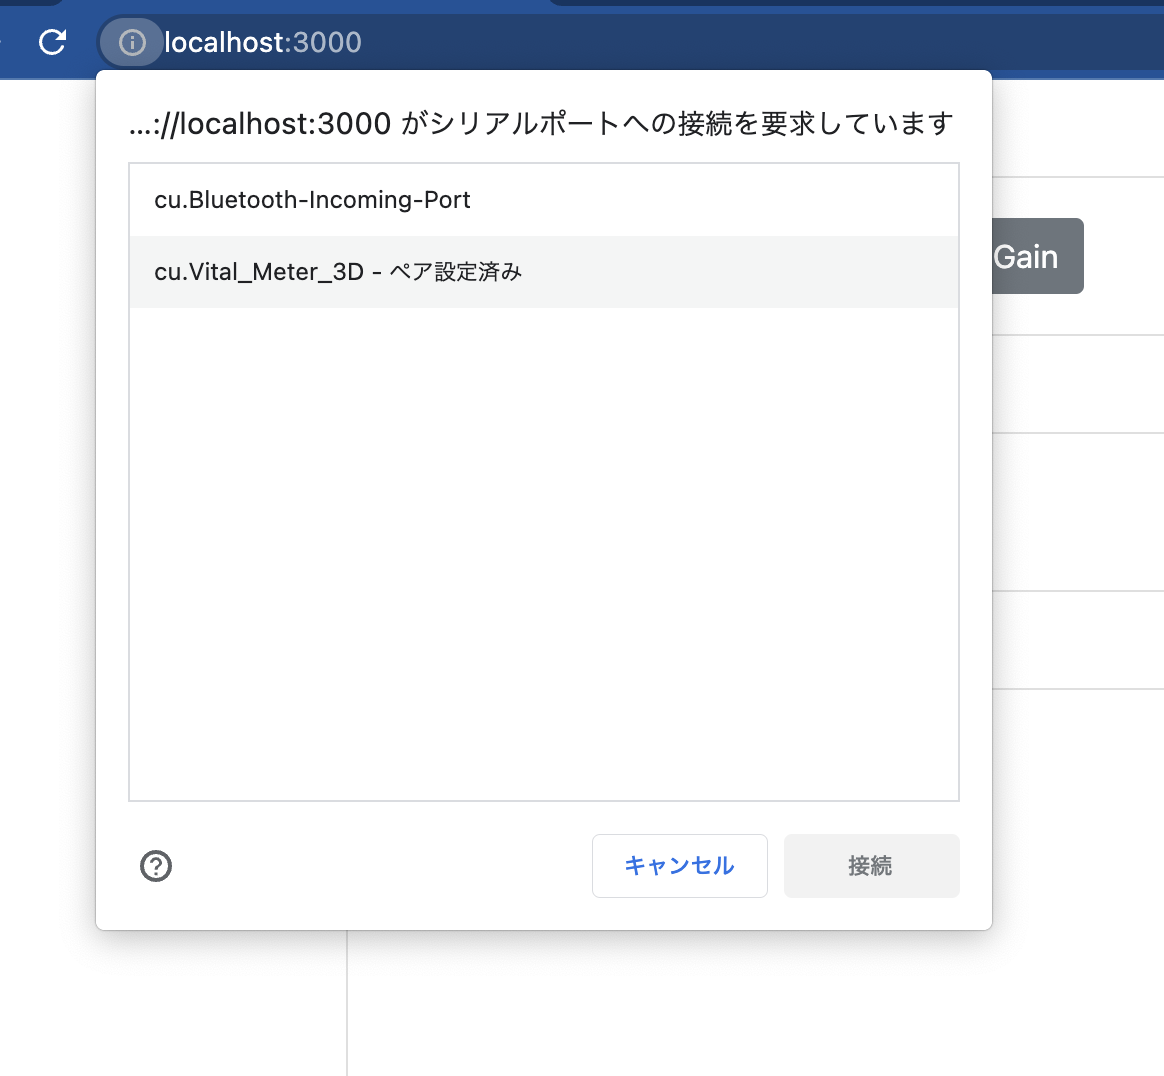
\includegraphics[width=50mm]{img/connectconfirm.png}
    \end{center}
    \caption{容積脈波計の接続画面}
    \label{fig:connectconfirm}
  \end{minipage}
\end{figure}

センサが接続されるとPreviewのフィールドに波形が表示される.波形が安定したことを確認して開始ボタンをクリックすると記録したBVPを保存するファイルを選択するダイアログが表示される.このシステムでは,BVPの計測データが大量になることからメモリ上に保存せずファイルに直接書き出す方式を採用している.通常のWebアプリケーションではファイルへの逐次書き出しが許可されていないため,いくつかのブラウザで実験的に実装されているFile System API\cite{filesystemapi}を使用してこれを可能にした.

BVPの記録を終了した後,分析ボタンをクリックすると脈波解析エンジンにデータが送られ,結果が図\ref{fig:uxgraph1}のように時系列で可視化される.RRIとANB(HFLF)は高いほどストレスが高く,LLE(Lyapunov)は低いほどストレスが高いことを表す.

\begin{figure}[htbp]
  \begin{minipage}{\hsize}
    \begin{center}
       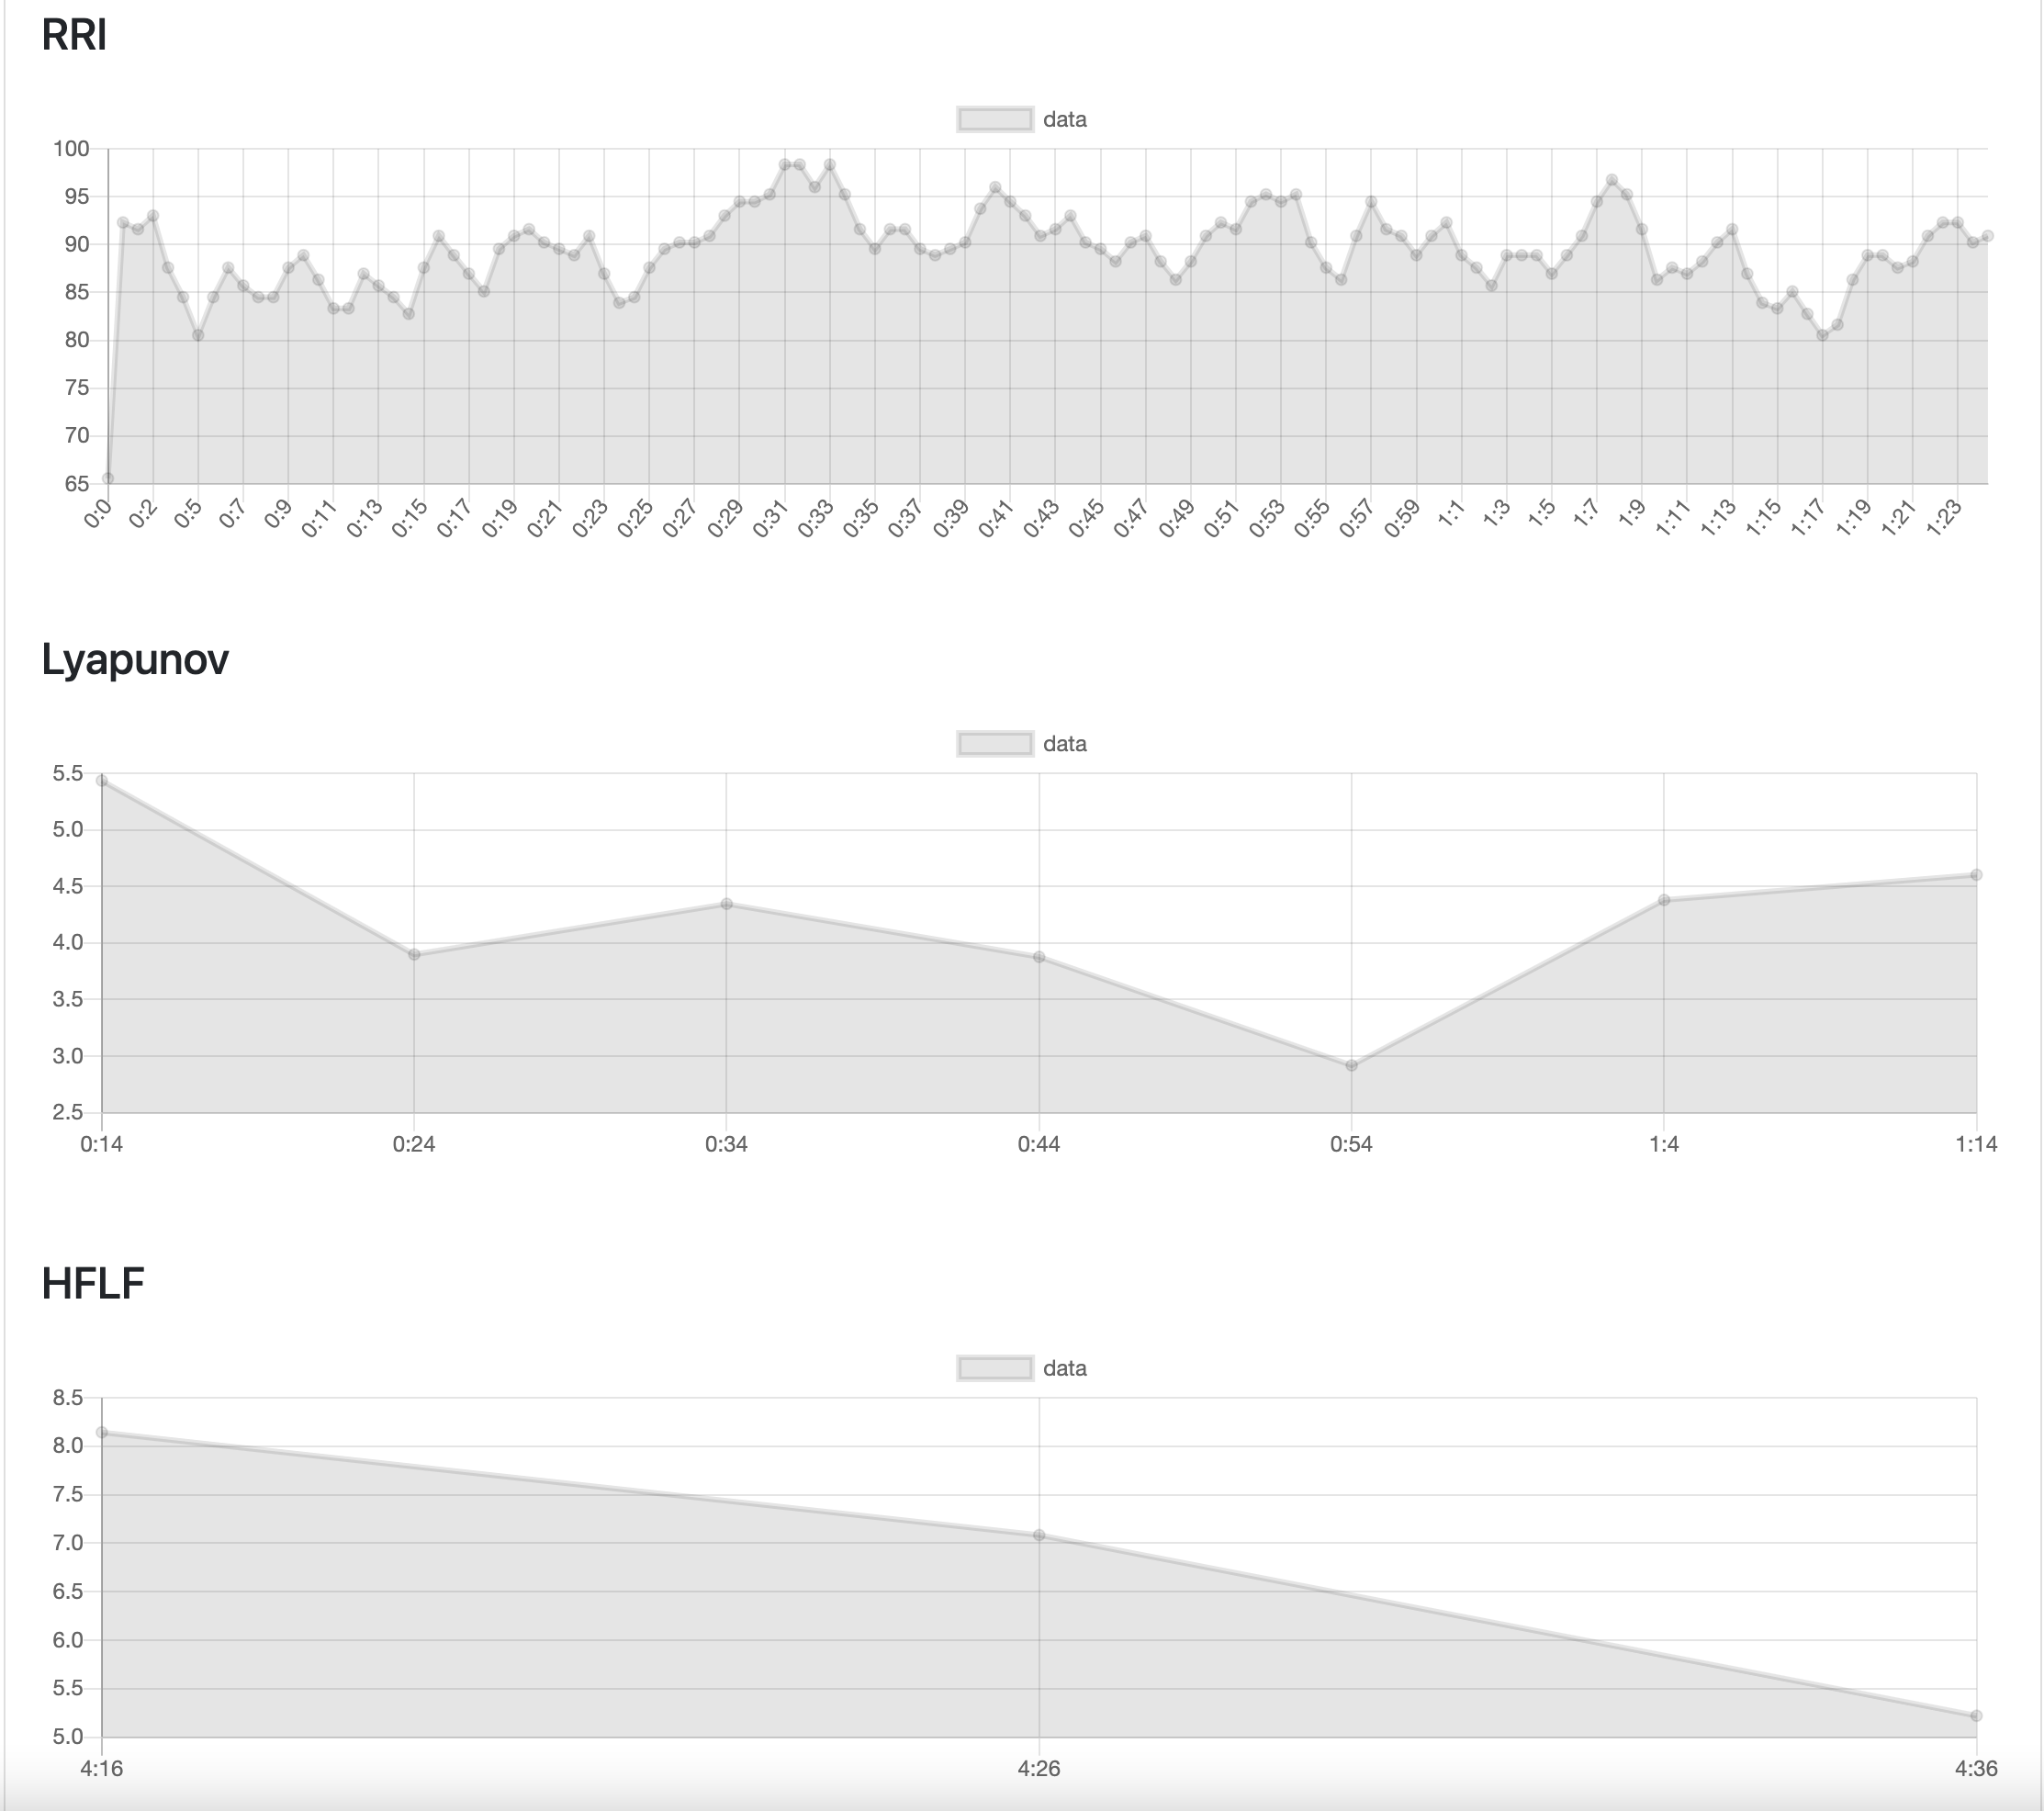
\includegraphics[width=100mm]{img/uxgraph1}
    \end{center}
    \caption{RRI,LLE,ANBの推移の表示画面}
    \label{fig:uxgraph1}
  \end{minipage}
\end{figure}

BVPの計測と同時に操作画面のスクリーンキャプチャや第三者視点での動画を収録し,それらの動画とストレスの値を関連付けることで,どの操作をしているときにストレスが高くなったのか,あるいはストレスが低かったのかを明らかにすることができる.
図\ref{fig:eventmap}
%詳しく書く

\begin{figure}[htbp]
  \begin{minipage}{\hsize}
    \begin{center}
       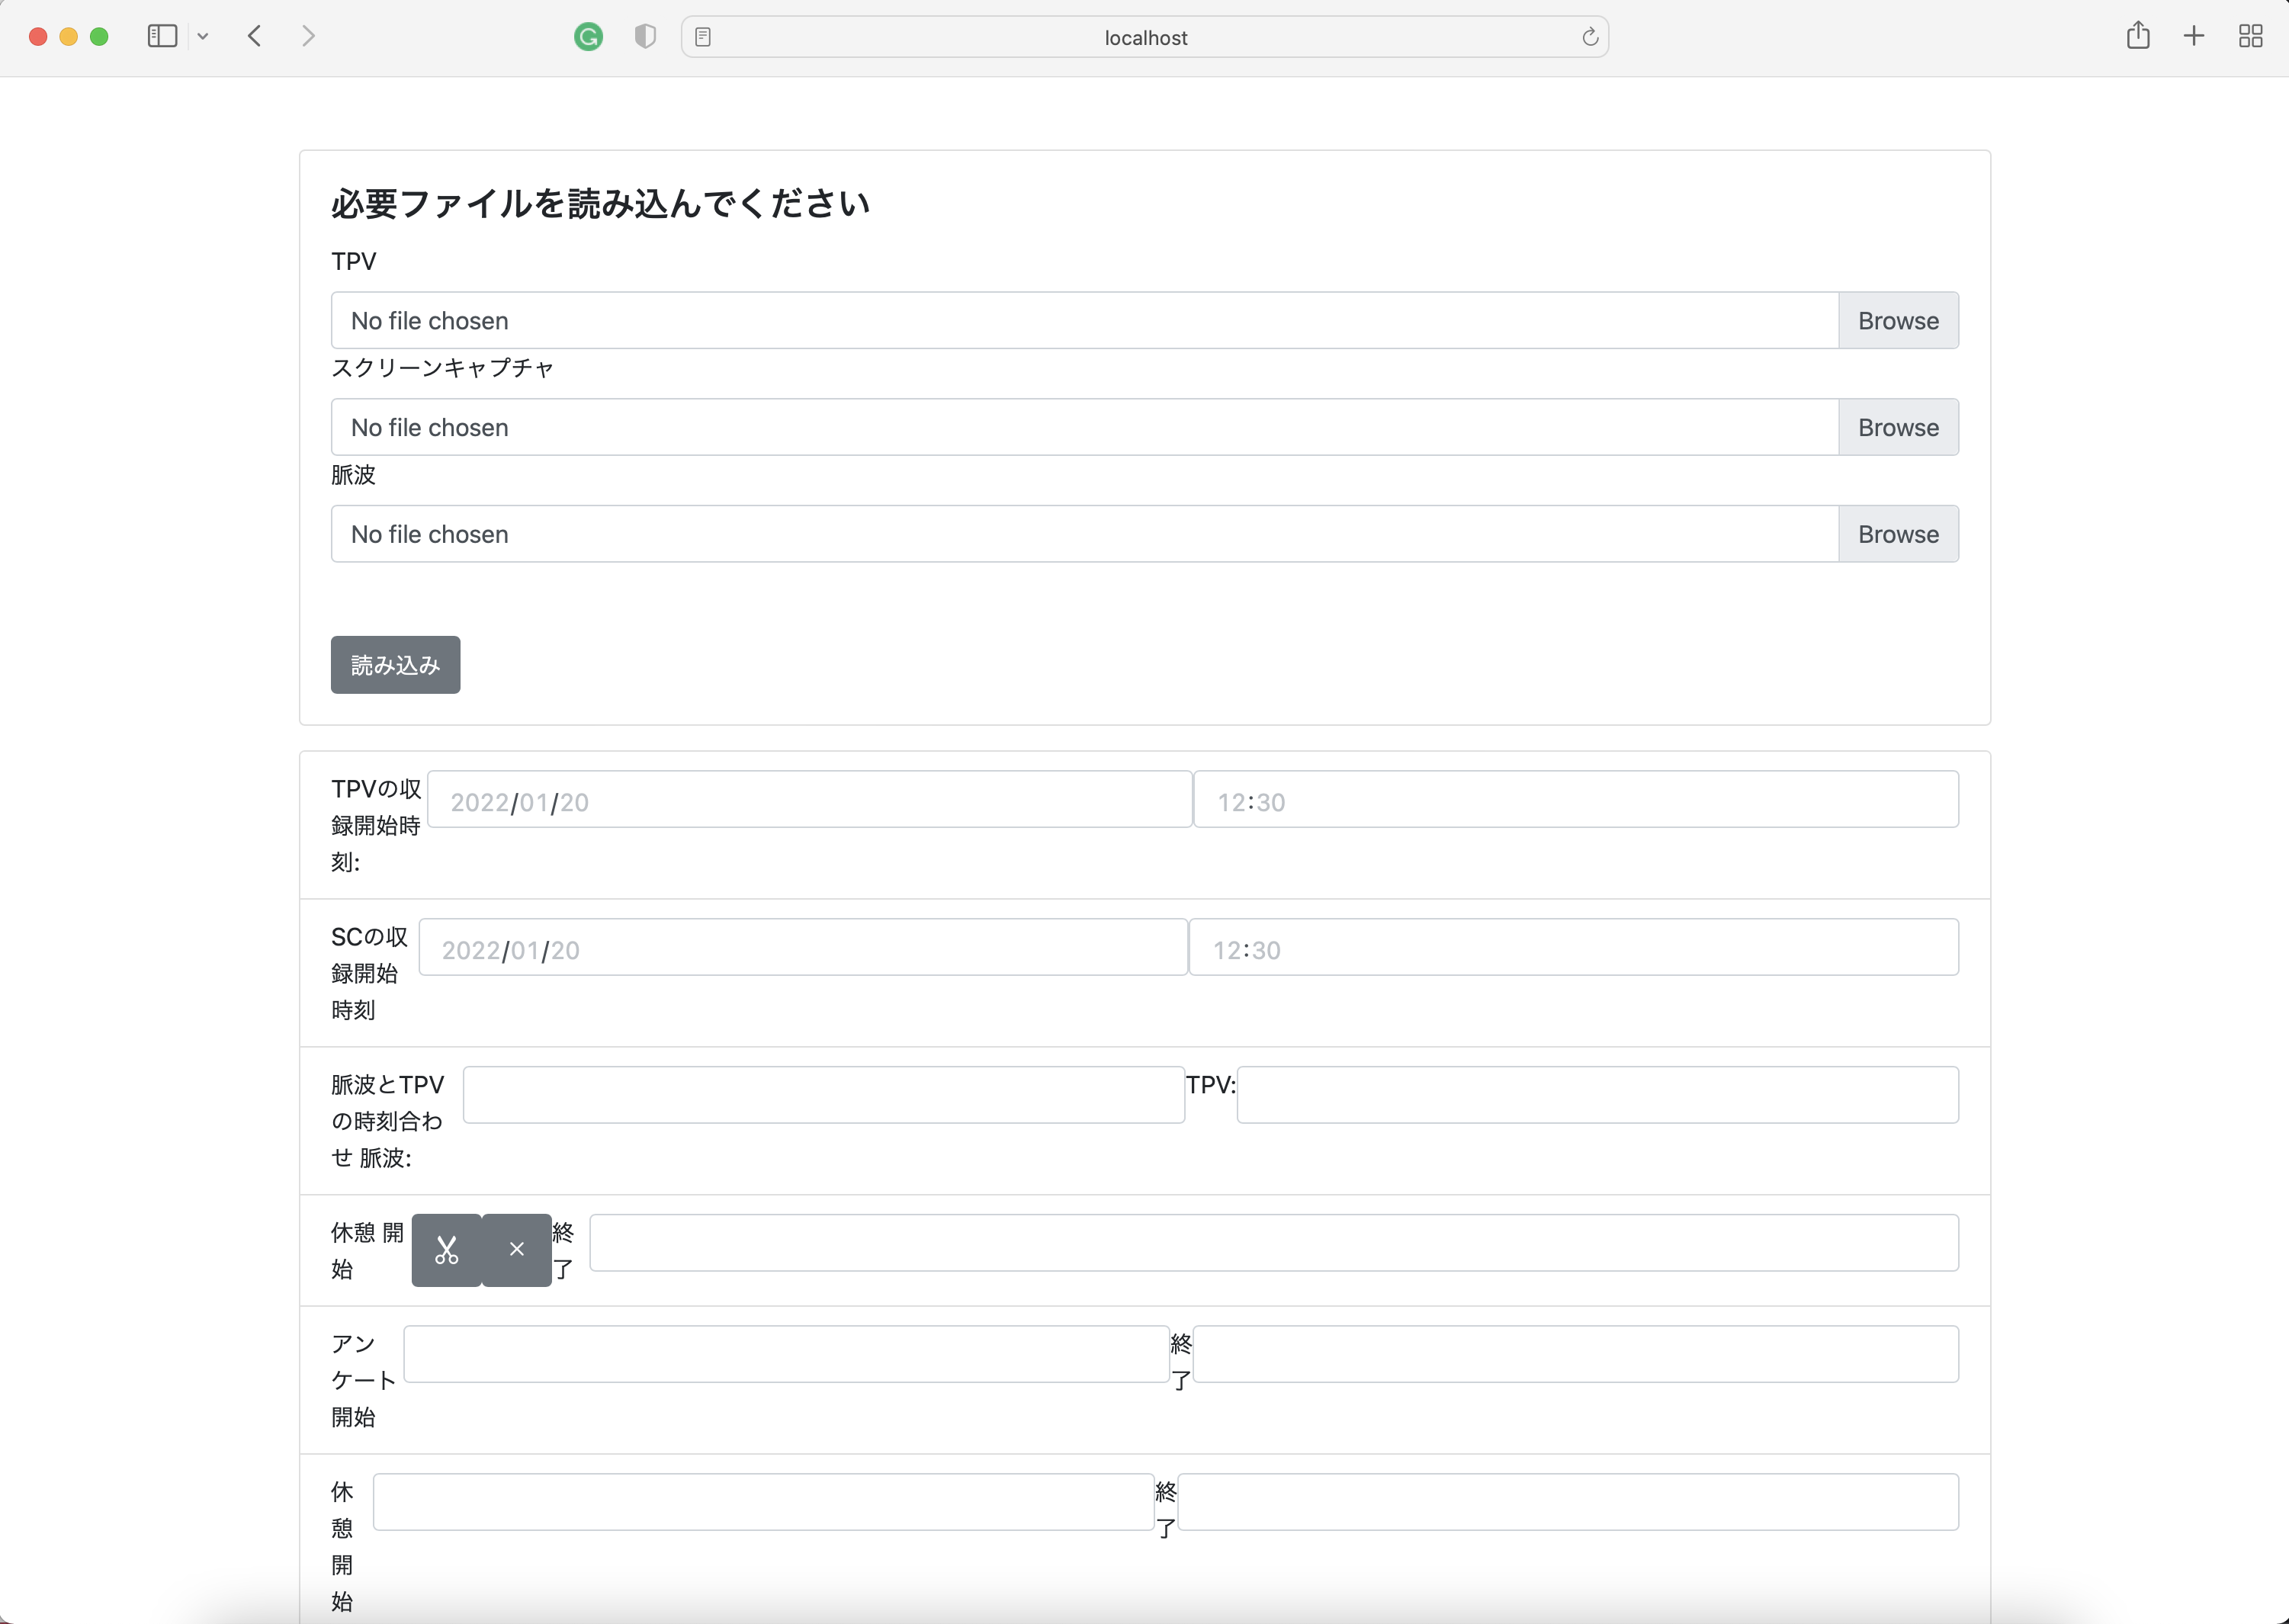
\includegraphics[width=100mm]{img/eventmap}
    \end{center}
    \caption{イベントのタイミング入力画面}
    \label{fig:eventmap}
  \end{minipage}
\end{figure}

\section{妥当性検討実験の計画}

2021年11月から12月に48名の大学生を対象に実験を行った.被験者の平均年齢は20.5歳($SD=1.66$),生物学的性の内訳は男子23名,女子25名であった.

\subsection{実験マテリアルの開発}

\begin{figure}[htbp]
  \begin{minipage}{0.5\hsize}
    \begin{center}
       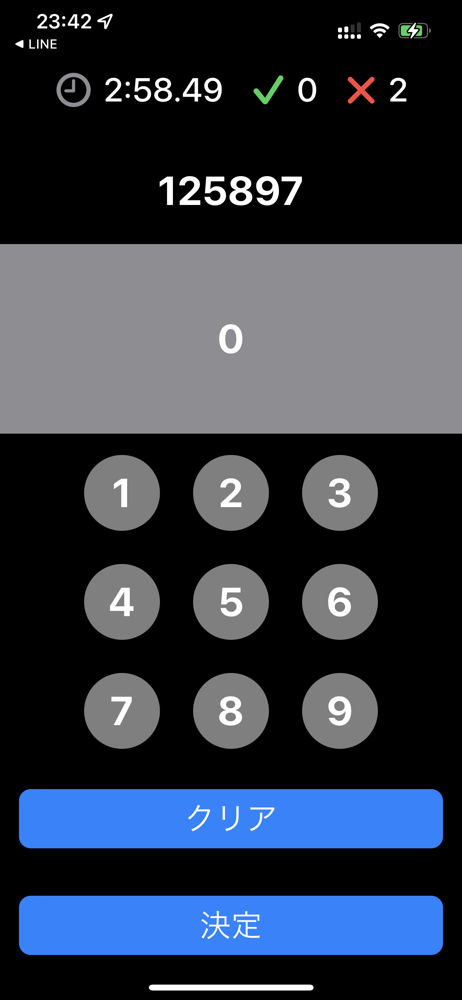
\includegraphics[width=40mm]{img/new1.png}
    \end{center}
    \caption{実験A(テンキー)の画面}
    \label{fig:tenkey}
  \end{minipage}
  \begin{minipage}{0.5\hsize}
    \begin{center}
       
\includegraphics[width=40mm]{img/new2.png}
    \end{center}
    \caption{実験B(ドラッグ)の画面}
    \label{fig:drag}
  \end{minipage}
\end{figure}

\subsection{タスクの実施}

\subsection{容積脈波(BVP)の計測と動画の収録}

\begin{figure}[htbp]
  \begin{minipage}{\hsize}
    \begin{center}
       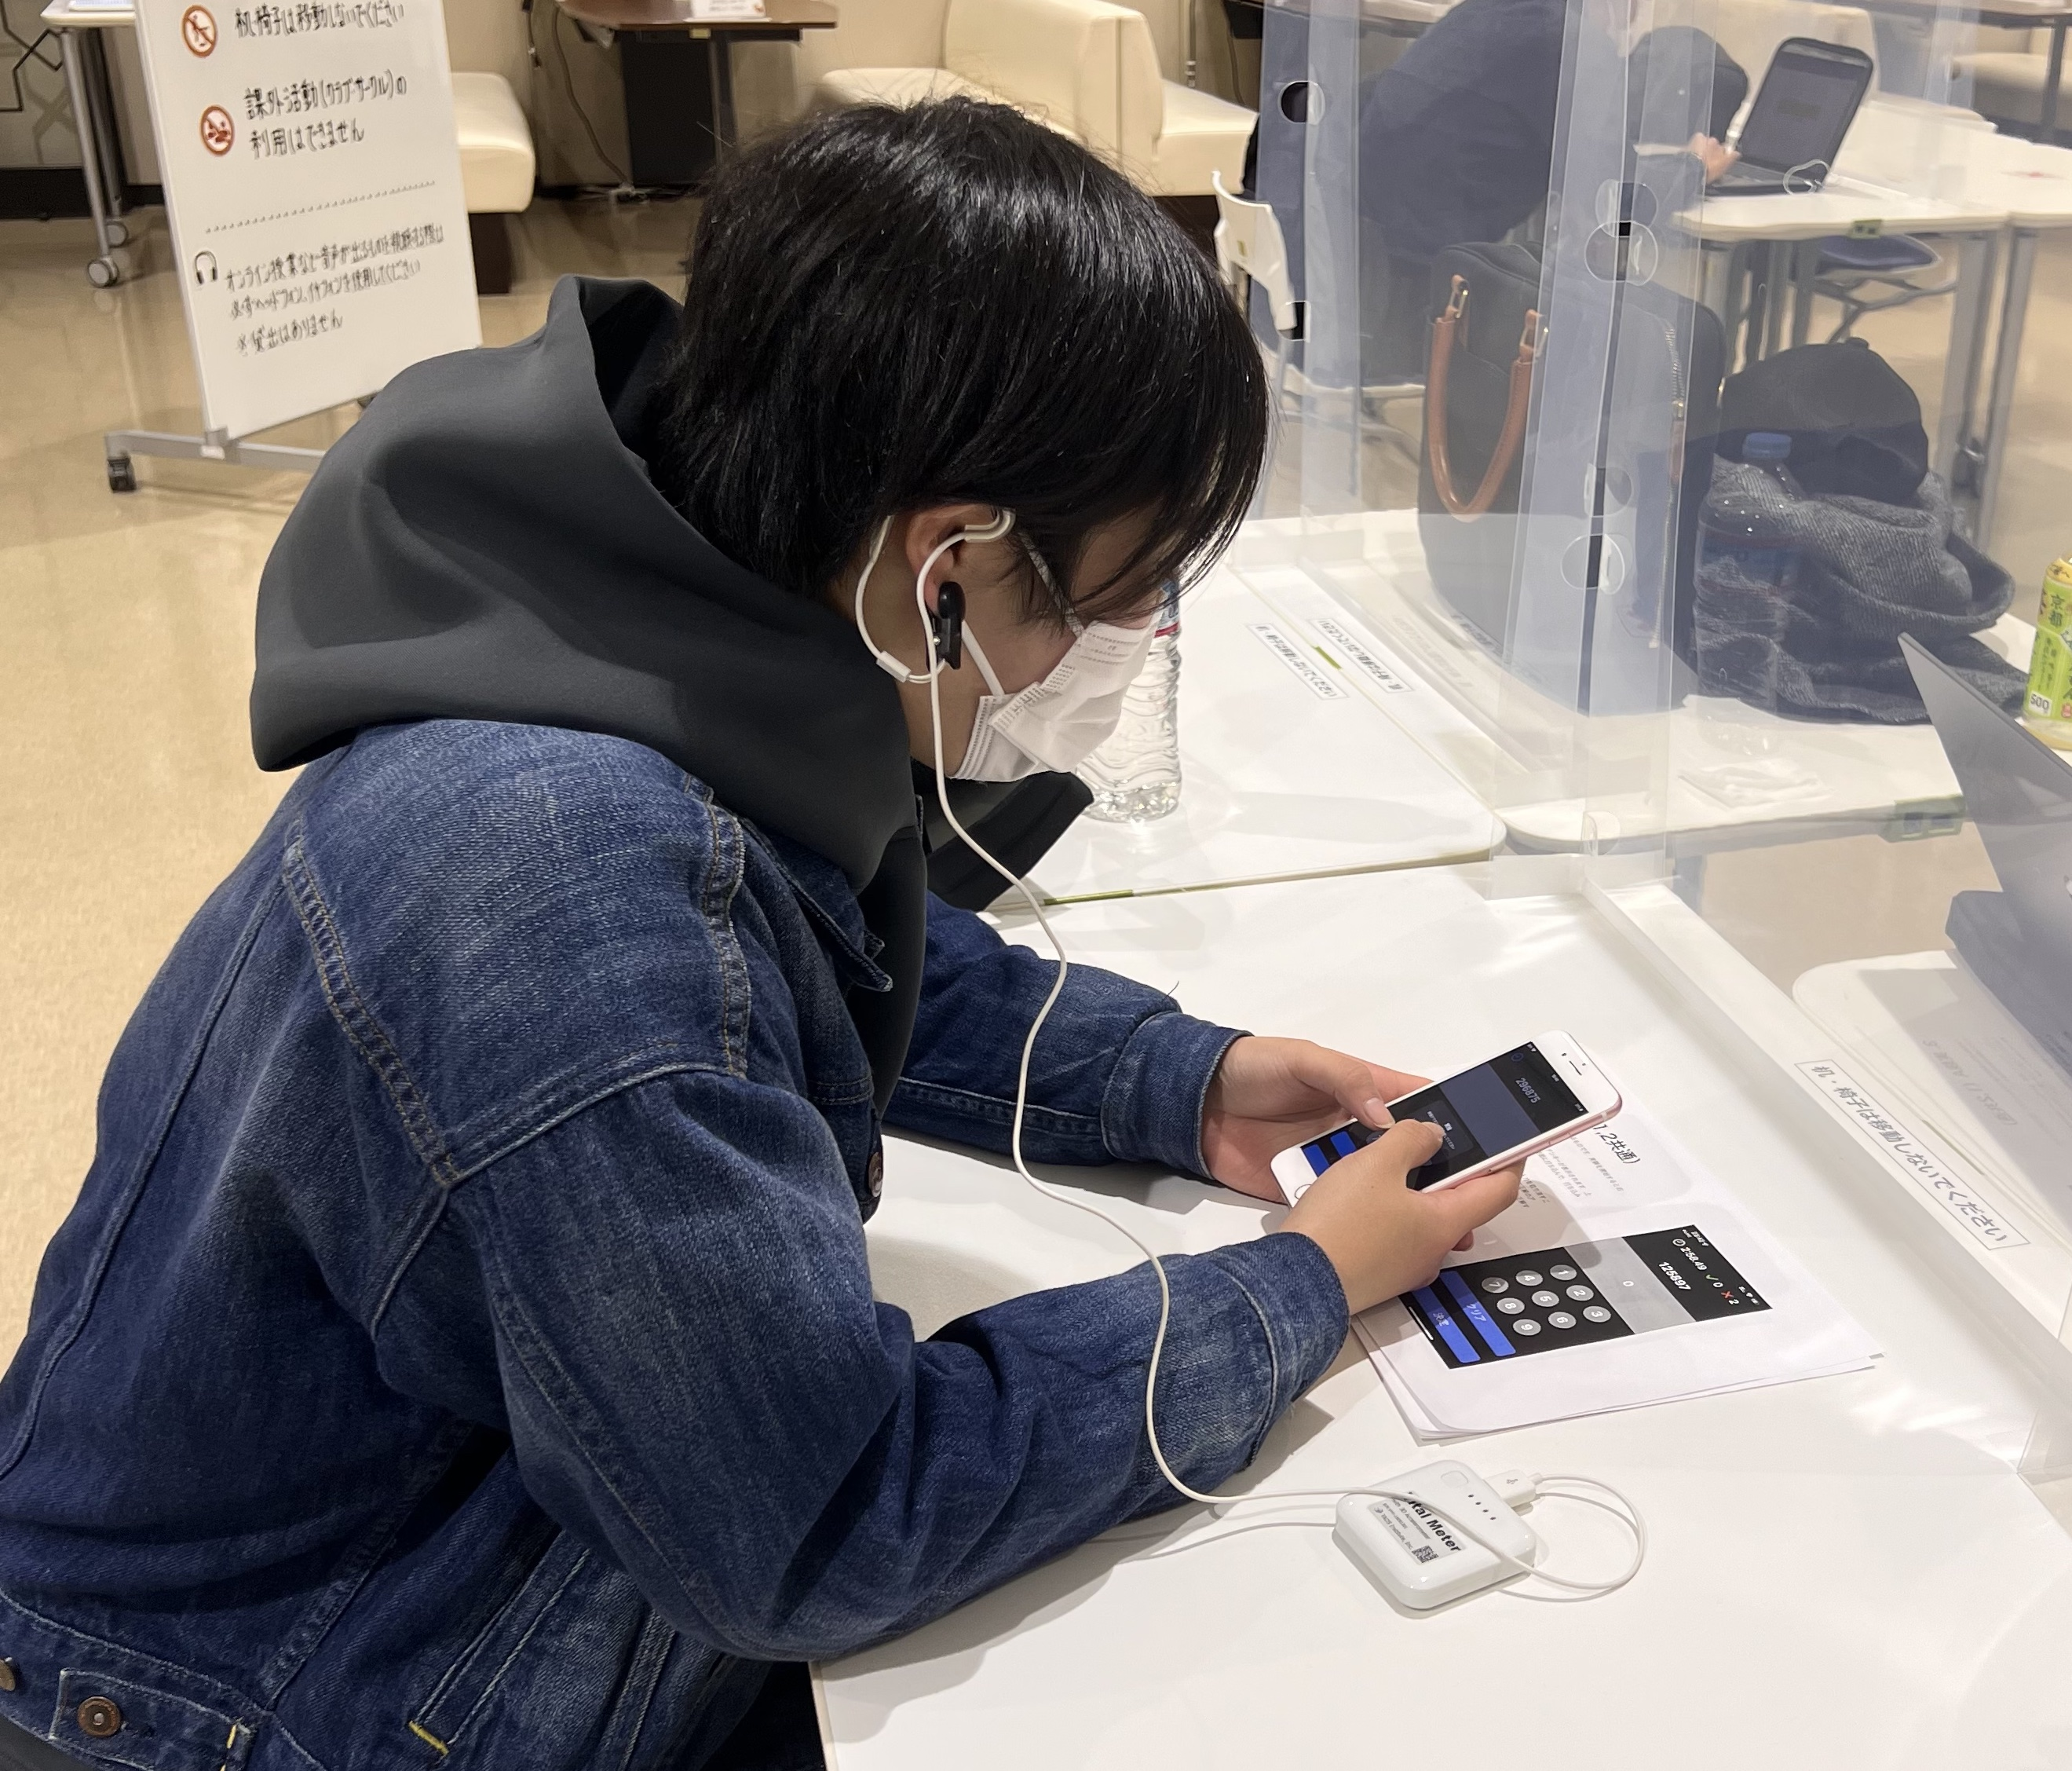
\includegraphics[width=100mm]{img/experience.jpg}
    \end{center}
    \caption{実験の様子}
    \label{fig:observe}
  \end{minipage}
\end{figure}

\subsection{アンケートの実施}
\cite{stressquestionare}

\section{実験の結果}

\begin{table}[htbp]
\centering
\scalebox{0.65}{
\begin{tabular}{llllllllllllllll}
\hline
\multirow{2}{*}{ID} & \multirow{2}{*}{A-1} & \multirow{2}{*}{A-2} & \multirow{2}{*}{B-1} & \multirow{2}{*}{B-2} & \multirow{2}{*}{C} & \multirow{2}{*}{年齢(歳)} & \multirow{2}{*}{性別} & \multirow{2}{*}{就寝時刻} & \multirow{2}{*}{起床時刻} & \multirow{2}{*}{(1)} & \multirow{2}{*}{(2)} & \multicolumn{4}{l}{最近のストレス反応} \\ \cline{13-16} 
                    &                      &                      &                      &                      &                    &                        &                     &                       &                       &                      &                      & (3)   & (4)   & (5)   & (6)   \\ \hline
1                   & 1                    & 2                    & 3                    & 4                    & 1                  & 22                     & F                   & 1:30                  & 8:00                  & 1                    & 0                    & 中     & 低     & 中     & 中     \\
2                   & 1                    & 2                    & 4                    & 3                    & 1                  & 20                     & F                   & 23:00                 & 6:40                  & 1                    & 0                    & 中     & 低     & 低     & 低     \\
3                   & 1                    & 3                    & 2                    & 4                    & 1                  & 24                     & M                   & 23:00                 & 10:00                 & 1                    & 1                    & 稍高    & 低     & 中     & 中     \\
4                   & 1                    & 4                    & 2                    & 3                    & 1                  & 22                     & M                   & 3:00                  & 10:00                 & 0                    & 0                    & 低     & 低     & 低     & 低     \\
5                   & 1                    & 3                    & 4                    & 2                    & 1                  & 18                     & M                   & 23:30                 & 8:30                  & 0                    & 0                    & 低     & 低     & 稍高    & 中     \\
6                   & 1                    & 4                    & 3                    & 2                    & 1                  & 22                     & M                   & 3:00                  & 8:00                  & 1                    & 0                    & 中     & 中     & 中     & 中     \\
7                   & 2                    & 1                    & 3                    & 4                    & 1                  & 22                     & F                   & 2:00                  & 7:30                  & 0                    & 0                    & 稍高    & 低     & 稍高    & 中     \\
8                   & 2                    & 1                    & 4                    & 3                    & 1                  & 22                     & M                   & 1:30                  & 11:30                 & 0                    & 0                    & 低     & 低     & 低     & 低     \\
9                   & 3                    & 1                    & 2                    & 4                    & 1                  & 21                     & M                   & 1:30                  & 9:30                  & 0                    & 0                    & 低     & 低     & 低     & 低     \\
10                  & 4                    & 1                    & 2                    & 3                    & 1                  & 21                     & M                   & 0:30                  & 9:30                  & 0                    & 0                    & 低     & 低     & 低     & 低     \\
11                  & 3                    & 1                    & 4                    & 2                    & 1                  & 19                     & M                   & 1:00                  & 4:50                  & 0                    & 0                    & 稍高    & 中     & 低     & 中     \\
12                  & 4                    & 1                    & 3                    & 2                    & 1                  & 21                     & M                   & 3:30                  & 10:55                 & 0                    & 0                    & 低     & 低     & 低     & 低     \\
13                  & 2                    & 3                    & 1                    & 4                    & 1                  & 18                     & M                   & 1:22                  & 7:30                  & 0                    & 0                    & 中     & 低     & 低     & 低     \\
14                  & 2                    & 4                    & 1                    & 3                    & 1                  & 19                     & M                   & 1:00                  & 9:00                  & 1                    & 0                    & 低     & 中     & 低     & 低     \\
15                  & 3                    & 2                    & 1                    & 4                    & 1                  & 19                     & F                   & 1:30                  & 9:00                  & 1                    & 0                    & 低     & 低     & 低     & 低     \\
16                  & 4                    & 2                    & 1                    & 3                    & 1                  & 19                     & M                   & 6:00                  & 12:15                 & 0                    & 0                    & 稍高    & 稍高    & 高     & 高     \\
17                  & 4                    & 3                    & 1                    & 2                    & 1                  & 22                     & F                   & 1:00                  & 7:00                  & 1                    & 0                    & 低     & 低     & 低     & 低     \\
18                  & 2                    & 3                    & 4                    & 1                    & 1                  & 18                     & M                   & 1:30                  & 7:15                  & 0                    & 0                    & 低     & 低     & 中     & 低     \\
19                  & 2                    & 4                    & 3                    & 1                    & 1                  & 22                     & F                   & 0:30                  & 7:30                  & 0                    & 0                    & 中     & 低     & 低     & 低     \\
20                  & 3                    & 2                    & 4                    & 1                    & 1                  & 19                     & M                   & 0:00                  & 6:30                  & 0                    & 0                    & 中     & 低     & 中     & 中     \\
21                  & 4                    & 2                    & 3                    & 1                    & 1                  & 18                     & F                   & 12:00                 & 9:30                  & 0                    & 0                    & 低     & 低     & 中     & 低     \\
22                  & 3                    & 4                    & 2                    & 1                    & 1                  & 19                     & M                   & 2:20                  & 11:00                 & 0                    & 0                    & 中     & 中     & 低     & 低     \\
23                  & 4                    & 3                    & 2                    & 1                    & 1                  & 18                     & F                   & 1:00                  & 11:00                 & 0                    & 0                    & 中     & 中     & 中     & 中     \\
24                  & 1                    & 2                    & 3                    & 4                    & 2                  & 19                     & M                   & 2:00                  & 8:30                  & 0                    & 0                    & 高     & 中     & 高     & 高     \\
25                  & 1                    & 2                    & 4                    & 3                    & 2                  & 22                     & F                   & 1:40                  & 10:30                 & 0                    & 0                    & 低     & 低     & 低     & 低     \\
26                  & 1                    & 3                    & 2                    & 4                    & 2                  & 21                     & F                   & 4:30                  & 10:00                 & 0                    & 0                    & 低     & 低     & 低     & 低     \\
27                  & 1                    & 4                    & 2                    & 3                    & 2                  & 22                     & F                   & 3:00                  & 11:00                 & 1                    & 0                    & 中     & 低     & 低     & 低     \\
28                  & 1                    & 3                    & 4                    & 2                    & 2                  & 22                     & M                   & 23:30                 & 13:30                 & 1                    & 0                    & 低     & 中     & 中     & 中     \\
29                  & 1                    & 4                    & 3                    & 2                    & 2                  & 22                     & F                   & 2:30                  & 9:30                  & 0                    & 0                    & 低     & 低     & 中     & 低     \\
30                  & 3                    & 4                    & 1                    & 2                    & 2                  & 21                     & F                   & 3:30                  & 11:00                 & 0                    & 1                    & 稍高    & 低     & 低     & 低     \\
31                  & 2                    & 1                    & 3                    & 4                    & 2                  & 18                     & M                   & 2:00                  & 9:00                  & 1                    & 1                    & 低     & 低     & 中     & 中     \\
32                  & 2                    & 1                    & 4                    & 3                    & 2                  & 19                     & M                   & 1:00                  & 8:00                  & 0                    & 0                    & 低     & 低     & 中     & 低     \\
33                  & 3                    & 1                    & 2                    & 4                    & 2                  & 22                     & F                   & 0:30                  & 8:00                  & 0                    & 0                    & 高     & 中     & 低     & 稍高    \\
34                  & 4                    & 1                    & 2                    & 3                    & 2                  & 21                     & F                   & 0:45                  & 8:30                  & 1                    & 0                    & 中     & 稍高    & 低     & 中     \\
35                  & 3                    & 1                    & 4                    & 2                    & 2                  & 21                     & M                   & 1:00                  & 9:00                  & 0                    & 0                    & 稍高    & 中     & 中     & 稍高    \\
36                  & 4                    & 1                    & 3                    & 2                    & 2                  & 23                     & F                   & 19:00                 & 3:00                  & 0                    & 0                    & 高     & 低     & 稍高    & 稍高    \\
37                  & 2                    & 3                    & 1                    & 4                    & 2                  & 22                     & F                   & 1:00                  & 7:20                  & 1                    & 0                    & 低     & 低     & 低     & 低     \\
38                  & 2                    & 4                    & 1                    & 3                    & 2                  & 21                     & F                   & 2:00                  & 7:30                  & 1                    & 0                    & 低     & 低     & 中     & 低     \\
39                  & 3                    & 2                    & 1                    & 4                    & 2                  & 21                     & M                   & 1:00                  & 8:00                  & 0                    & 0                    & 低     & 低     & 中     & 低     \\
40                  & 4                    & 2                    & 1                    & 3                    & 2                  & 22                     & F                   & 1:15                  & 8:10                  &                      &                      & 高     & 高     & 高     & 高     \\
41                  & 3                    & 4                    & 1                    & 2                    & 2                  & 18                     & M                   & 1:10                  & 7:40                  & 0                    & 0                    & 低     & 低     & 中     & 低     \\
42                  & 4                    & 3                    & 1                    & 2                    & 2                  & 19                     & M                   & 0:00                  & 7:10                  & 0                    & 0                    & 中     & 低     & 中     & 低     \\
43                  & 2                    & 3                    & 4                    & 1                    & 2                  & 19                     & F                   & 12:00                 & 6:00                  & 1                    & 0                    & 中     & 低     & 中     & 低     \\
44                  & 2                    & 4                    & 3                    & 1                    & 2                  & 22                     & F                   & 4:30                  & 9:30                  & 0                    & 0                    & 中     & 低     & 低     & 低     \\
45                  & 3                    & 4                    & 2                    & 1                    & 2                  & 18                     & F                   & 1:00                  & 8:30                  & 0                    & 0                    & 中     & 低     & 稍高    & 中     \\
46                  & 4                    & 2                    & 3                    & 1                    & 2                  & 19                     & F                   & 12:00                 & 7:15                  & 0                    & 0                    & 低     & 低     & 低     & 低     \\
47                  & 3                    & 2                    & 4                    & 1                    & 2                  & 22                     & F                   & 23:50                 & 8:00                  & 1                    & 0                    & 中     & 低     & 高     & 中     \\
48                  & 4                    & 3                    & 2                    & 1                    & 2                  & 21                     & F                   & 23:30                 & 7:30                  & 0                    & 0                    & 中     & 低     & 低     & 低     \\ \hline
\multicolumn{16}{l}{A-1,A-2,B-1,B-2はそれぞれ実験A Bad UI,Good UI,実験 B Bad UI,Good UI.番号は実験の実施順を示す.}                                                                                                                                                                                                                     \\
\multicolumn{16}{l}{Cはアンケートの形式を示す(問題毎ページ遷移は1,セクション毎ページ遷移は2)}                                                                                                                                                                                                                                                      \\
\multicolumn{16}{l}{(1):職業・専攻・趣味がデザインや芸術に関連している (あてはまる場合は1)}                                                                                                                                                                                                                                                      \\
\multicolumn{16}{l}{(2):職業・専攻・趣味がソフトウェアのフロントエンドの開発に関連している(あてはまる場合は1)}                                                                                                                                                                                                                                             \\
\multicolumn{16}{l}{(3):抑うつ・不安 (4):不機嫌・怒り (5):無気力 (6):合計}                                                                                                                                                                                                                                                        
\end{tabular}
}
\caption{時系列UX評価検証実験: 被験者の概要}
\label{table:exp2result1}
\end{table}


\section{実験の分析}

\begin{table}[htbp]
\centering
\begin{tabular}{llrlr}
\hline
    & \multicolumn{2}{l}{実験A}                             & \multicolumn{2}{l}{実験B}                             \\ \cline{2-5} 
    & Good UI(件)                & \multicolumn{1}{l}{Bad UI(件)} & Good UI(件)                & \multicolumn{1}{l}{Bad UI(件)} \\ \hline
肯定的 & \multicolumn{1}{r}{16} & 1                          & \multicolumn{1}{r}{22} & 3                          \\
否定的 & \multicolumn{1}{r}{}   & 34                         & \multicolumn{1}{r}{1}  & 34                         \\ \hline
\end{tabular}
\caption{時系列UX評価システム検証実験:マテリアルに対する肯定肯定の別}
\label{table:negaposi}
\end{table}

\begin{table}[htbp]
\centering
\begin{tabular}{lrrrrr}
\hline
            & \multicolumn{1}{l}{実験A}     & \multicolumn{1}{l}{}       & \multicolumn{1}{l}{実験B}     & \multicolumn{1}{l}{}       & \multicolumn{1}{l}{\multirow{2}{*}{合計(件)}} \\ \cline{2-5}
            & \multicolumn{1}{l}{Good UI(件)} & \multicolumn{1}{l}{Bad UI(件)} & \multicolumn{1}{l}{Good UI(件)} & \multicolumn{1}{l}{Bad UI(件)} & \multicolumn{1}{l}{}                    \\ \hline
スムーズ        & 7                           &                            & 8                           &                            & 15                                      \\
反応が良い       & 3                           &                            & 5                           &                            & 8                                       \\
快適だった       & 3                           &                            & 5                           &                            & 8                                       \\
正常だった       & 2                           &                            & 1                           &                            & 3                                       \\
ゲーム性があった    &                             & 1                          &                             & 1                          & 2                                       \\
達成感があった     &                             &                            &                             & 2                          & 2                                       \\
順調だった       &                             &                            & 2                           &                            & 2                                       \\
ストレスを感じなかった & 1                           &                            & 1                           &                            & 2                                       \\
挑戦したくなった    & 1                           &                            &                             &                            & 1                                       \\
ミスが無かった     &                             &                            & 1                           &                            & 1                                       \\
多く正解できた     & 1                           &                            &                             &                            & 1                                       \\
楽しかった       & 1                           &                            &                             &                            & 1                                       \\ \hline
\end{tabular}
\caption{時系列UX評価システム検証実験:マテリアルに対する肯定的意見の内訳}
\label{table:posi}
\end{table}

\begin{table}[htbp]
\centering
\begin{tabular}{lrrrrr}
\hline
             & \multicolumn{1}{l}{実験A}     & \multicolumn{1}{l}{}       & \multicolumn{1}{l}{実験B}     & \multicolumn{1}{l}{}       & \multicolumn{1}{l}{\multirow{2}{*}{合計(件)}} \\ \cline{2-5}
             & \multicolumn{1}{l}{Good UI(件)} & \multicolumn{1}{l}{Bad UI(件)} & \multicolumn{1}{l}{Good UI(件)} & \multicolumn{1}{l}{Bad UI(件)} & \multicolumn{1}{l}{}                    \\ \hline
反応が悪かった      &                             & 25                         &                             & 23                         & 48                                      \\
難しかった        &                             & 4                          &                             & 8                          & 12                                      \\
ストレスを感じた     &                             & 5                          &                             & 5                          & 10                                      \\
ミスがあった       &                             & 8                          &                             & 2                          & 10                                      \\
焦った          &                             & 6                          &                             & 1                          & 7                                       \\
悔しかった        &                             &                            &                             & 5                          & 5                                       \\
作業のように感じた    &                             &                            & 1                           & 1                          & 2                                       \\
動揺した         &                             & 2                          &                             &                            & 2                                       \\
煩わしかった       &                             & 1                          &                             & 1                          & 2                                       \\
モヤモヤした       &                             &                            &                             & 1                          & 1                                       \\
何がダメかわからなかった &                             &                            &                             & 1                          & 1                                       \\
困った          &                             &                            &                             & 1                          & 1                                       \\
慣れなかった       &                             & 1                          &                             &                            & 1                                       \\
疲労を感じた       &                             &                            &                             & 1                          & 1                                      \\ \hline
\end{tabular}
\caption{時系列UX評価システム検証実験:マテリアルに対する否定的意見の内訳}
\label{table:nega}
\end{table}


\section{実験の考察}

